\subsubsection*{UMap}

\paragraph{Overview}

UMap is a user level library providing a high performance mmap-like
interface that can be tuned to application needs without requiring OS
customization or impacting system configuration. UMap enables
applications to interact with out-of-core data sets as if in memory,
and to configure parameters such as page buffer size and page size on
a per-application basis.

Leadership supercomputers feature a diversity of storage, from
node-local persistent memory and NVMe SSDs to network-interconnected
flash memory and HDD. Interacting with large persistent data sources
is critical to exascale applications that harness the power of data
analytics and machine learning. The UMap user-level library enables
user-space page management of data located in the memory/storage
hierarchy. By providing a memory map interface, applications can
interact with large data sets as if in memory. As a user level
library, a UMap page fault handler can be easily adapted to access
patterns in applications and to storage characteristics, reducing latency
and improving performance.

\paragraph{Key Challenges}

As ECP applications transition to include ML and data analytics as
integral components of workflows, persistent memories and low latency
storage devices offer new alternatives to hold portions of very large
global data sets within the fabric of the computing system. These new
applications drive new access patterns, i.e. read-dominated analysis
of observational or simulation data rather than write-mostly
checkpoints. The combination of new technologies (byte addressable,
very low latency, asymmetric read/write latency), new insertion points
(node local, Top of Rack or other intermediate storage, global FS,
external distributed storage servers), and new applications (in-situ
analytics, experimental $+$ simulation data analysis, ML batched data
sets) present challenges both to the traditional memory/storage
dichotomy as well as to traditional HPC I/O libraries tailored to
checkpoint transmission.

\paragraph{Solution Strategy}

We prioritize four design choices for UMap based on surveying
realistic use cases. First, we choose to implement UMap as a
user-level library so that it can maintain compatibility with the
fast-moving Linux kernel without the need to track and modify for
frequent kernel updates. Also, we employ the recent \texttt{userfaultfd} 
mechanism, rather than the signal handling + callback function approach
to reduce overhead and performance variance in multi-threaded
applications. Third, we target an adaptive solution that sustains
performance even at high concurrency for data-intensive applications,
which often employ a large number of threads for hiding data access
latency. Our design pays particular consideration on load imbalance
among service threads to improve the utilization of shared resources
even when data accesses to pages are skewed. UMap dynamically balances
workloads among all service threads to eliminate bottleneck on serving
hot pages. Finally, for flexible and portable tuning on different
computing systems, UMap provides both API and environmental controls
to enable configurable page sizes, eviction strategy,
application-specific prefetching, and detailed diagnosis information to the
programmer. The UMap software architecture is shown in Figure
\ref{fig:umaparch}.

\begin{figure}[t]
        \centering
        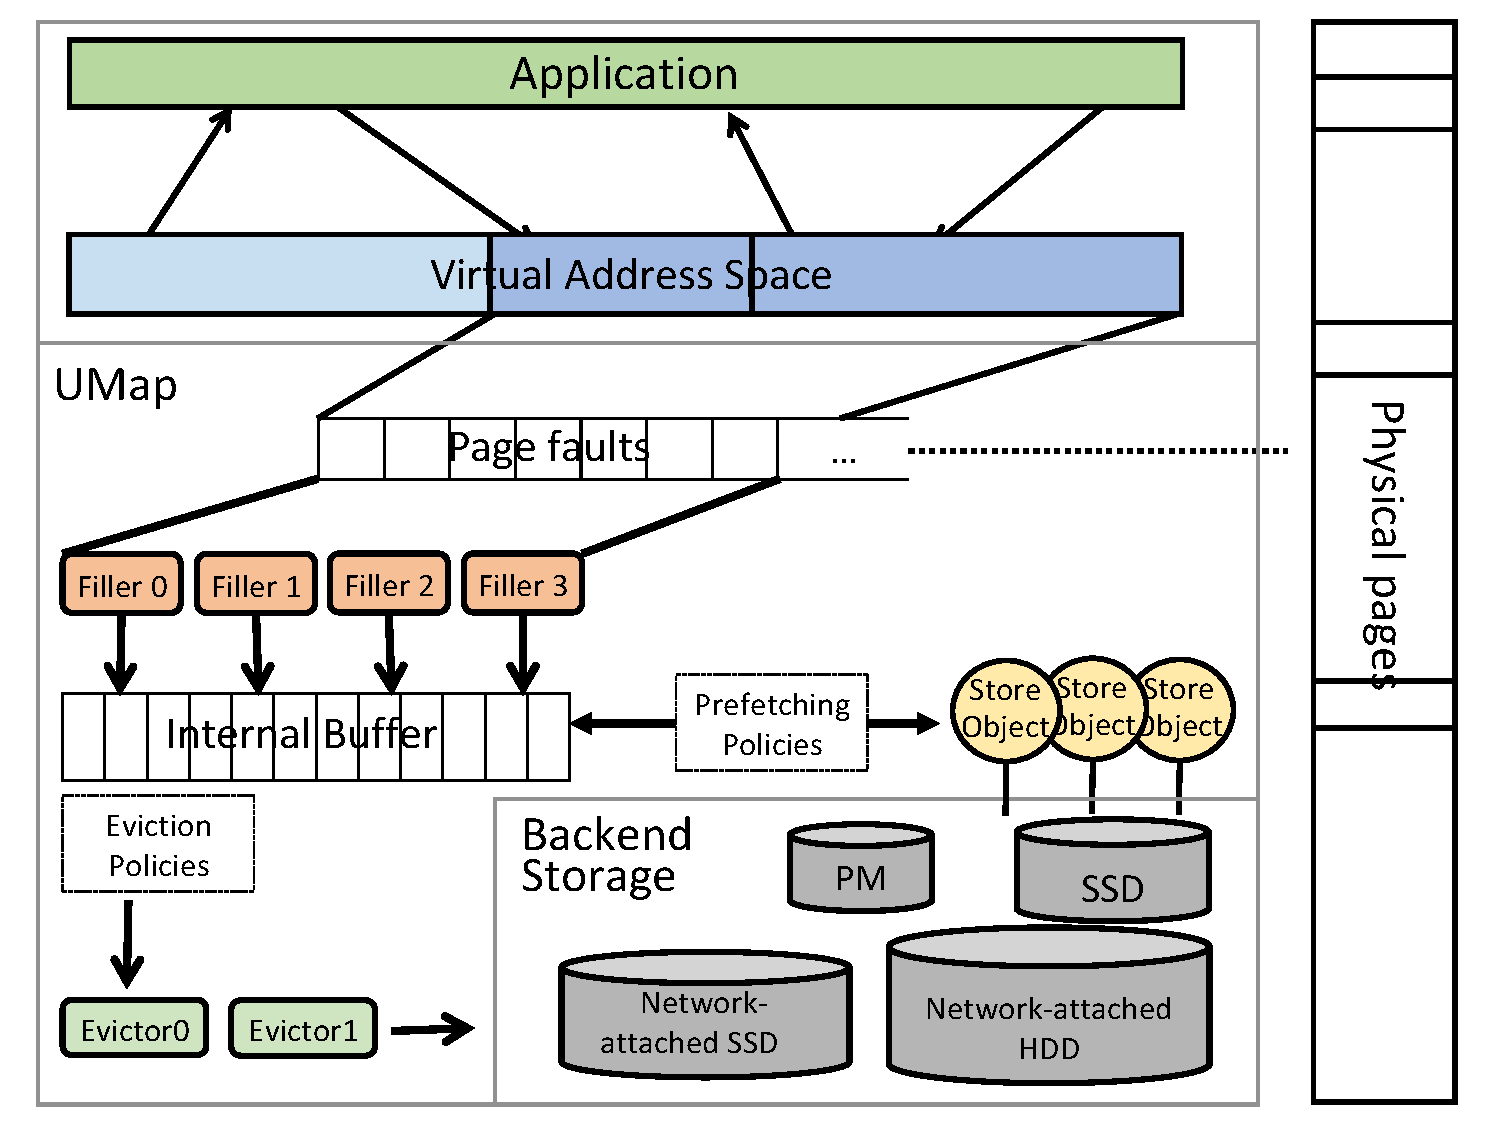
\includegraphics[scale = 0.5]{projects/2.3.1-PMR/2.3.1.19-Argo-PowerSteering/umap-arch}
        \caption{UMap Handler architecture}
        \label{fig:umaparch}
\end{figure}

\paragraph{Recent Progress}

In recent months, we have released MP-UMap, providing multi-process
support for the UMap facility. MP-UMap enables multiple processes on a
compute node to share the UMap page buffer so that pages accessed from
a mapped file are accessible to MPI ranks on the same node. 

The LLNL UMap team demonstrated graph analysis algorithms based on
graph traversal that use the UMap handler.  By integrating with SICM’s
persistent memory C++ allocator called Metall into UMap, the UMap
handler provides memory mapped access to very large graphs dynamically
allocaetd and stored in binary form in one or more file(s). The
algorithm suite consists of a dynamic graph construction benchmark,
breadth-first search, connected components, and the ExaGraph miniVite
benchmark.

An adaptive buffer management scheme was added to UMap to monitor and
react at runtime to adjust the page buffer size. With this
optimization, the page buffer can grow and shrink to reflect memory
space availability changes.

A paper on UMap was published in IEEE Transactions on Parallel and
Distributed Systems:  Peng, I.B., Gokhale, M., Youssef, K., Iwabuchi, K. and Pearce, R., 2021. Enabling Scalable and Extensible Memory-mapped Datastores in Userspace. doi: 10.1109/TPDS.2021.3086302

\paragraph{Next Steps}
In the coming year, we plan to continue outreach to application teams
within ECP and in the science/data community. This includes
collaboration with the Umpire team, and with graph algorithm
developers. We will integrate UMap with Umpire to give applications a
common API to manage multiple sorts of memories including persistent
memory through UMap and main CPU and GPU memory resources. The
Exagraph collaboration will map persistent data such as binary format
graphs and intermediate data structures through UMap using the
SparseStore and Metall.

